%%%%%%%%%%%%%%%%%%%%%%%%%%%%%%%%%%%%%%%%%%%%%%%%%%%%%%%%%%% Author - Varad Meru
%% tex source file for ML Homeworks
%%%%%%%%%%%%%%%%%%%%%%%%%%%%%%%%%%%%%%%%%%%%%%%%%%%%%%%%%
\documentclass[a4paper, 11pt]{article}

\usepackage[margin=1in]{geometry} % changes the margin
\usepackage{lipsum} % adds random text to check the formatting
\usepackage{hyperref} % adds hyperlink
\usepackage[framed,numbered,autolinebreaks,useliterate]{mcode}
\usepackage{subfigure}
\usepackage{graphicx}
\usepackage{enumerate}

\renewcommand{\thefootnote}{\fnsymbol{footnote}} % Changes the format of the footnotes superscripts

%%%%%%%%%%%%%%%%%%%%%%%%%%%%%%%%%%%%%%%%%%%%%%%%%%%%%%%%%
\begin{document}
\begin{noindent}
\large\textbf{Week 3} \hfill \textbf{Varad Meru} \\
\normalsize CS 273a - Introduction to Machine Learning (Winter '15)\footnote{\href{http://sli.ics.uci.edu/Classes/2015W-273a}{Website: http://sli.ics.uci.edu/Classes/2015W-273a}} \hfill Student \# 26648958 \\
Prof. Alex Ihler \hfill Due Date: 01/27/2015
\end{noindent}
\noindent\makebox[\linewidth]{\rule{\textwidth}{0.4pt}}

%%%%%%%%%%%%%%%%%%%%%%%%%%%%%%%%%%%%%%%%%%%%%%%%%%%%%%%%%
%%%%%%%%%%%%%%%%%%%%%%%%%%%%%%%%%%%%%%%%%%%%%%%%%%%%%%%%%
\begin{center}
\textbf{\Large{Homework 3}\footnote{Questions available at \href{http://sli.ics.uci.edu/Classes/2015W-273a?action=download\&upname=HW2.pdf}{http://sli.ics.uci.edu/Classes/2015W-273a?action=download\&upname=HW3.pdf}}\footnote{All the figures and listing numbers are auto-referred.}}\\
\end{center}
\vspace{-25pt}

%%%%%%%%%%%%%%%%%%%%%%%%%%%%%%%%%%%%%%%%%%%%%%%%%%%%%%%%%
%%%%%%%%%%%%%%%%%%%%%%%%%%%%%%%%%%%%%%%%%%%%%%%%%%%%%%%%%
%%%%%%%%%%%%%%%%%%%%%%%%%%%%%%%%%%%%%%%%%%%%%%%%%%%%%%%%%
\section*{Problem 1: Perceptron and Logistic Regression}
\vspace{-10pt}
\begin{enumerate}[(a)]
\item The scatter plot of the data is generated by code written in \autoref{lst:scatter}. The scatter plots generated can be seen in \autoref{fig:scatter}. From visual inspection, it can be seen that the data is linearly separable.

\vspace{-25pt}
\begin{lstlisting}[caption={Plotting the scatter plot},label={lst:scatter},numbers=left,escapeinside={@}{@}]
iris=load('data/iris.txt');     % load the text file
Y = iris(:,end);           % target value is last column
X = iris(:,1:end-1);       % features are other columns
features = char('Sepal length','Sepal width','Petal length','Petal width','Species');
features_short = char('SL','SW','PL','PW','SP');

% Vertically Splitting the dataset. Keeping the first 2 columns for the
% perceptron.
Xs = X(:,1:2);

% Shuffling and Rescaling X
[Xs Y] = shuffleData(Xs,Y);
Xs  = rescale(Xs);

% get class 0 vs 1
XA = Xs(Y<2,:); 
YA=Y(Y<2);
% get class 1 vs 2
XB = Xs(Y>0,:); 
YB=Y(Y>0);

%% Problem a
h=figure; scatter(XA(:,1), XA(:,2), 50, YA,'filled'); saveas(h,'scatter-classes1.jpg','jpg'); h=figure; scatter(XB(:,1), XB(:,2), 50, YB,'filled'); saveas(h,'scatter-classes2.jpg','jpg');
\end{lstlisting}

%%%%%%%%%%%%%%%%%%%%%%%%%%%%%%%%%%%%%%%%%%%%%%%%%%%%%%%%%
\item The \mcode{@logisticClassify2/plot2DLinear} is modified to present the decision boundary and can be seen in \autoref{lst:plot2d1}. The generated scatter plots can be seen in \autoref{fig:scatter2}.

\vspace{-20pt}
\begin{lstlisting}[caption={The \mcode{plot2DLinear()}},label={lst:plot2d1},numbers=left,escapeinside={@}{@}]
function plot2DLinear(obj, X, Y)
[n,d] = size(X);
if (d~=2) error('Sorry -- plot2DLogistic only works on 2D data...'); end;
  
%%% TODO: Fill in the rest of this function...
wts = getWeights(obj);
% LaTeX does not display the 'at' symbol
f = @@(x1, x2) wts(1) + wts(2)*x1 +wts(3)*x2;

scatter(X(:,1),X(:,2),50,Y,'filled');
hold on;
ezplot(f,[-3,3])
hold off;
\end{lstlisting}

\vspace{-25pt}
\begin{lstlisting}[caption={plotting using \mcode{plot2DLinear()}},label={lst:plot2d2},numbers=left,escapeinside={@}{@}]
%% Problem b
learner = logisticClassify2();
learner=setClasses(learner, unique(YA));
wts = [.5 1 -.25];
learner=setWeights(learner, wts);

h=figure;
plot2DLinear(learner,XA,YA);
saveas(h,'log1.jpg','jpg');

h=figure;
plot2DLinear(learner,XB,YB);
saveas(h,'log2.jpg','jpg');
\end{lstlisting}

%%%%%%%%%%%%%%%%%%%%%%%%%%%%%%%%%%%%%%%%%%%%%%%%%%%%%%%%%
\item The \mcode{predict()} function, given in \autoref{lst:predict}, would find the sign of the passed data points based on the function and weights assigned.
\vspace{-25pt}
\begin{lstlisting}[caption={\mcode{predict()} function},label={lst:predict},numbers=left,escapeinside={@}{@}]
function Yte = predict(obj,Xte)
% Yhat = predict(obj, X)  : make predictions on test data X
% (1) make predictions based on the sign of wts(1) + wts(2)*x(:,1) + ...
% (2) convert predictions to saved classes: Yte = obj.classes( [1 or 2] );
wts = getWeights(obj);
yhat = zeros(size(Xte,1),1);

% LaTeX does not display the 'at' symbol
f = @@(x1, x2) wts(1) + wts(2)*x1 + wts(3)*x2;

for i=1:size(Xte,1);
    x = sign(f(Xte(i,1),Xte(i,2)));
    yhat(i) = obj.classes(ceil((x+3)/2));
end;

Yte = yhat;
\end{lstlisting}
The \mcode{predict()} function is used to predict the possible classes and the error is computed using \mcode{errorTrain()}. The code can be seen in \autoref{lst:predict2}, along with the errors for the \mcode{XA} and \mcode{XB} sections of the data.
\vspace{-25pt}
\begin{lstlisting}[caption={Train and Test Error using the \mcode{predict()}},label={lst:predict2},numbers=left,escapeinside={@}{@}]
%% Problem c
yte = predict(learner,XA);
error = errorTrain(YA,yte);
% error = 0.0505
yte = predict(learner,XB);
error = errorTrain(YB,yte);
% error = 0.5455
\end{lstlisting}

\begin{figure}
\centering
\subfigure[Scatter Plot data of classes 0 and 1.]{
    \label{fig:scatter1}
    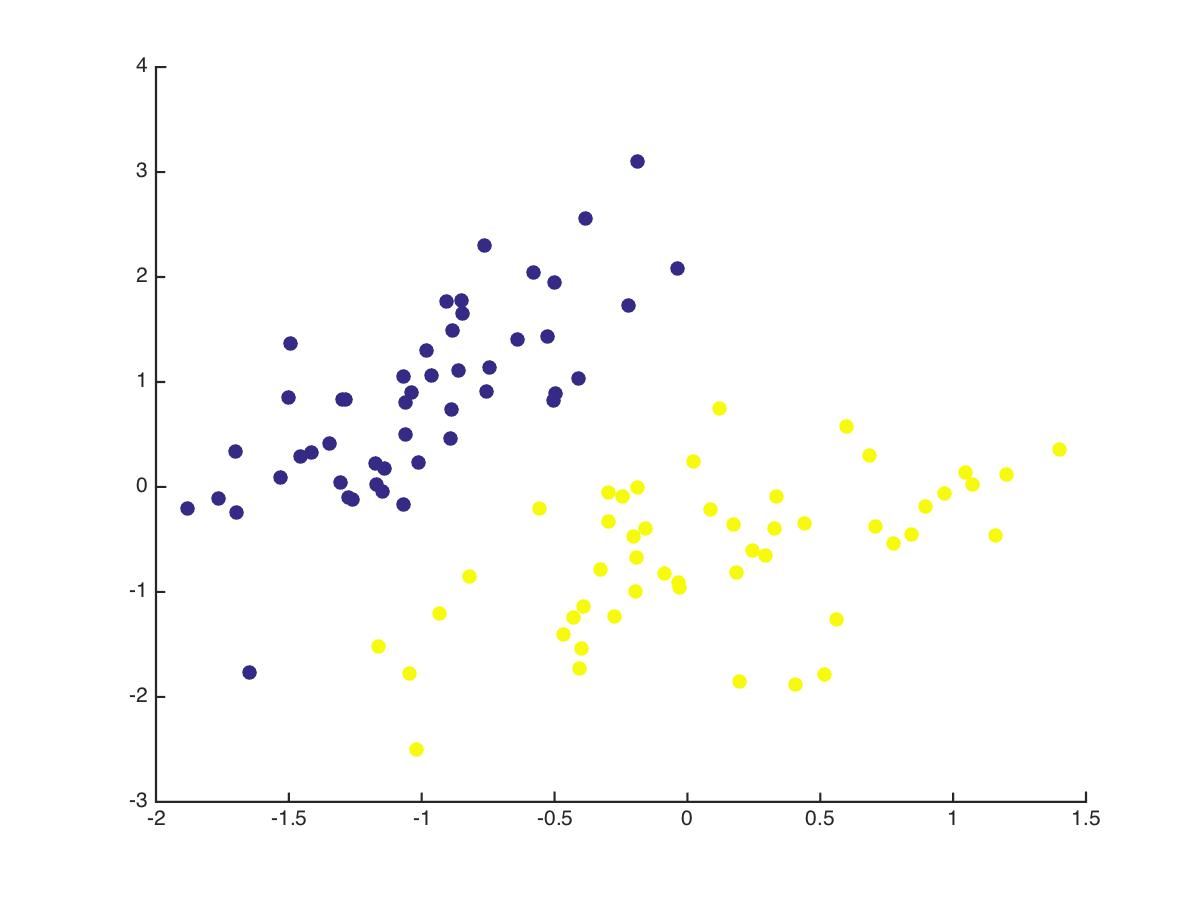
\includegraphics[scale=0.15]{scatter-classes1.jpg}
}
\subfigure[Scatter Plot data of classes 1 and 2.]{
    \label{fig:scatter2}
    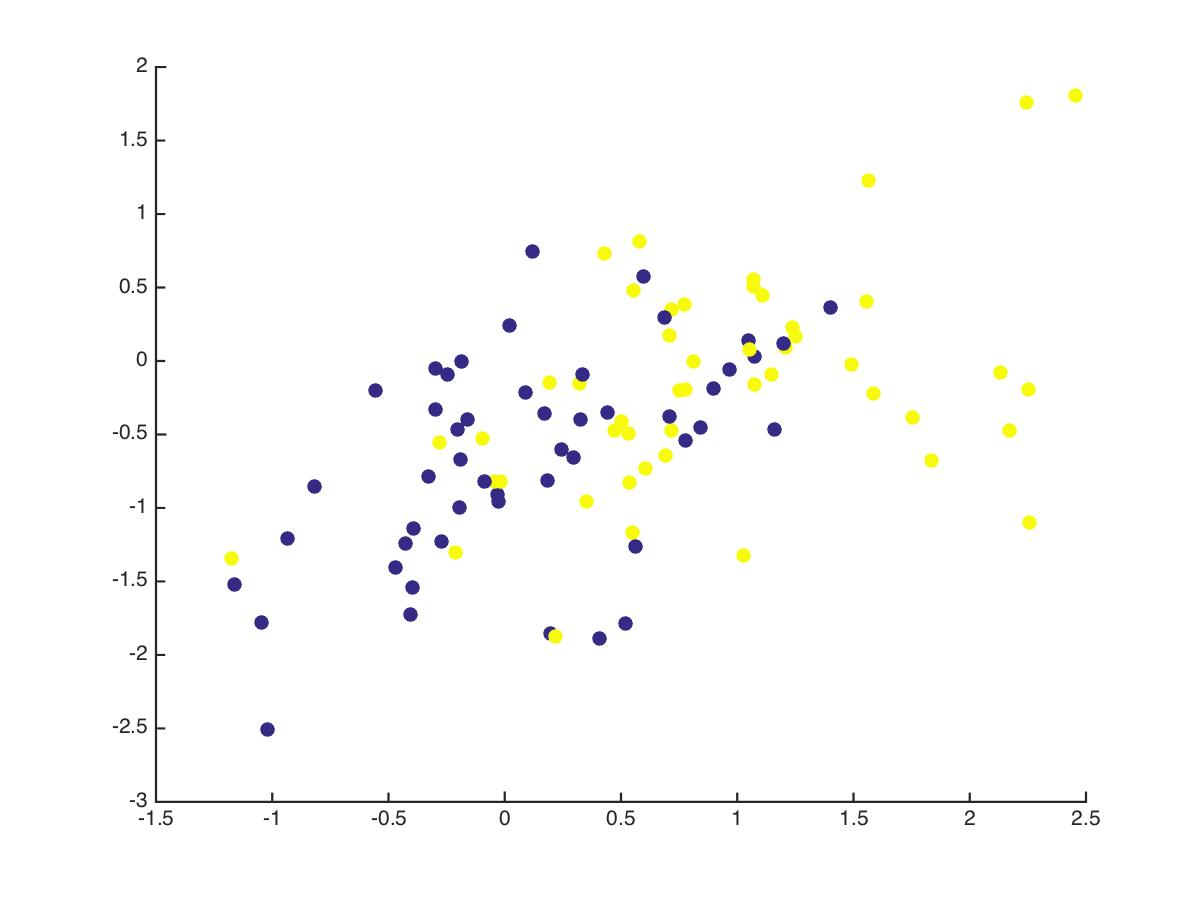
\includegraphics[scale=0.15]{scatter-classes2.jpg}
}
\caption[Scatter]{Scatter Plots of data}
\label{fig:scatter}
\end{figure}

\begin{figure}
\centering
\subfigure[Scatter Plot data of classes 0 and 1.]{
    \label{fig:scatter3}
    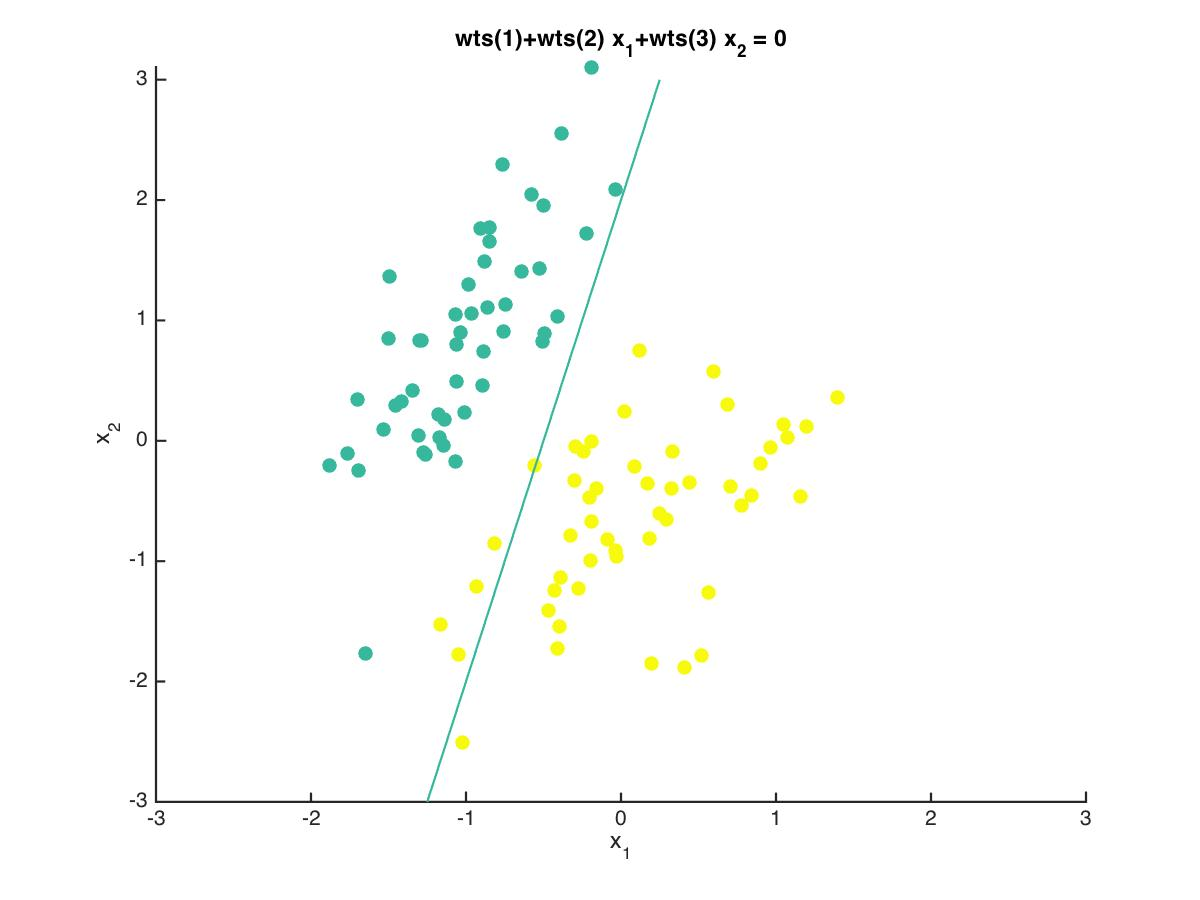
\includegraphics[scale=0.15]{log1.jpg}
}
\subfigure[Scatter Plot data of classes 1 and 2.]{
    \label{fig:scatter4}
    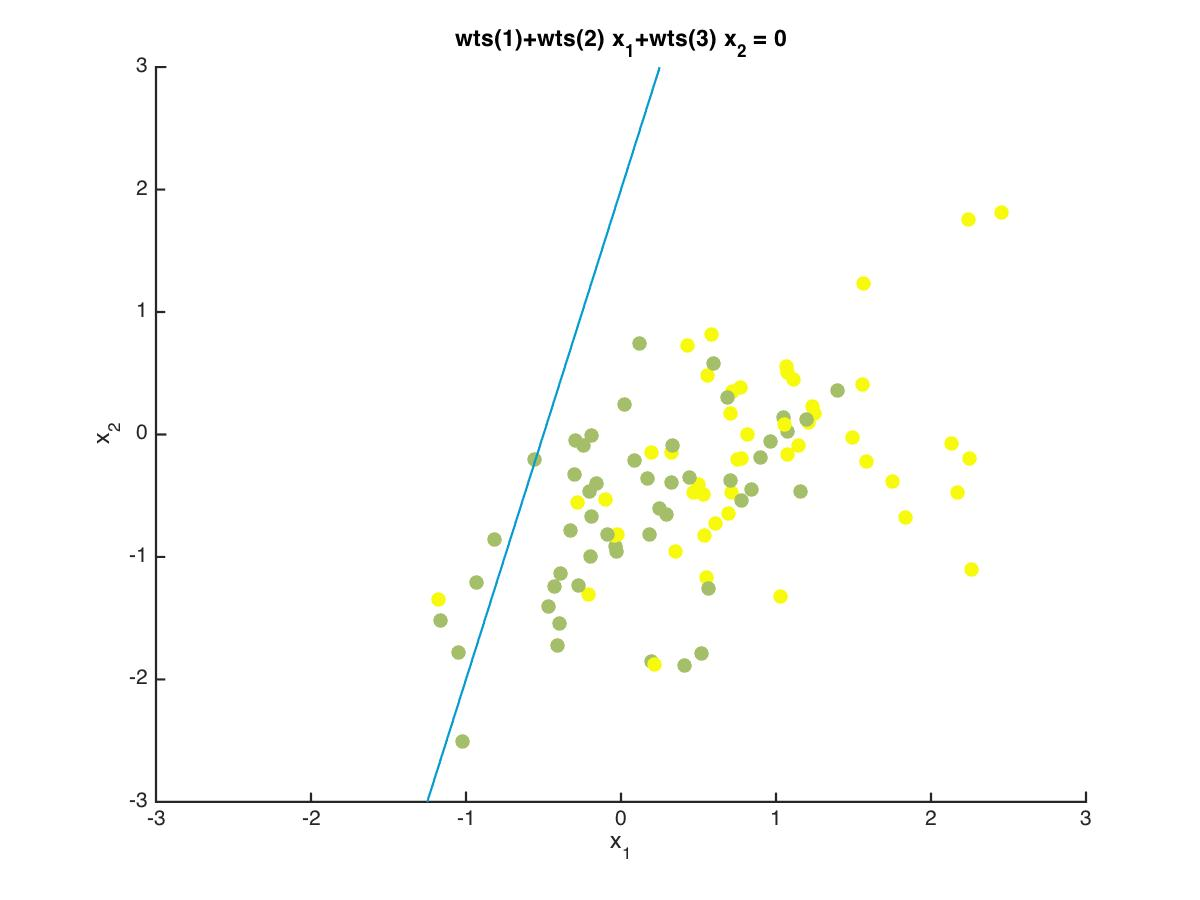
\includegraphics[scale=0.15]{log2.jpg}
}
\caption[Scatter]{Scatter Plots of data with the Perceptron Decision boundary for weights = [0.5 1 -0.25]}
\label{fig:scatter2}
\end{figure}
%%%%%%%%%%%%%%%%%%%%%%%%%%%%%%%%%%%%%%%%%%%%%%%%%%%%%%%%%
\item The derivation of the gradient is done my computing the \(\frac{\partial J_j(\theta)}{\partial \theta_i}\) over the surrogate loss for point \(j\) given by \(x^{(j)}, y^{(j)}\). The derivative is given \autoref{eqn:grad1}, where \(\sigma(z) = (1 + exp(z))^{-1}\) and \(z = \theta.x^{(j)T}\)

\begin{equation}
\frac{\partial J_j(\theta)}{\partial \theta_i} = x^{(j)}  (\sigma(z)-y^{(j)}) + 2.\alpha.\theta_{i}
\label{eqn:grad1}
\end{equation}

%$ (\sigma(z)-y^{(j)}).x^{(j)} + 2.\alpha.\theta_{i}$\\
%where $\sigma(z) = (1 + exp(z))^{-1}$ , where $z = \theta.x^{(j)T}$

%%%%%%%%%%%%%%%%%%%%%%%%%%%%%%%%%%%%%%%%%%%%%%%%%%%%%%%%%
\item I completed the \mcode{train()} function with the following changes
\begin{enumerate}[1.]
\item To compute the surrogate loss function at each iteration, I calculate the surrogate losses for each point and then compute the mean. (See \autoref{lst:train})
\item Computing the gradient and predictions of data point \(x^{(i)}, y^{(i)}\) is done using the \mcode{logistic()} function provided (See \autoref{lst:train}).
\item The gradient step derived in the 1(d) part of this question is computed in this step. This helps us to find the movement of the solution and direction required to reach near the optima (See \autoref{lst:train}).
\item The stopping condition is calculated and enforced at the end of the loop. It can be seen in \autoref{lst:train}.
\vspace{-25pt}
\begin{lstlisting}[caption={\mcode{train()} function snippet},label={lst:train},numbers=left,escapeinside={@}{@}]
while (~done) 
  step = stepsize/iter;               % update step-size and evaluate current loss values
  %Jsur(iter) = inf;   %%% TODO: compute surrogate (neg log likelihood) loss
  Jsur(iter) =mean( - Y .* log(logistic(obj, X)) - (1 - Y) .* log(1 - logistic(obj, X)) + reg * obj.wts * obj.wts');
  J01(iter) = err(obj,X,Yin);

  if (plotFlag), switch d,            % Plots to help with visualization
    case 1, fig(2); plot1DLinear(obj,X,Yin);  %  for 1D data we can display the data and the function
    case 2, fig(2); plot2DLinear(obj,X,Yin);  %  for 2D data, just the data and decision boundary
    otherwise, % no plot for higher dimensions... %  higher dimensions visualization is hard
  end; end;
  fig(1); semilogx(1:iter, Jsur(1:iter),'b-',1:iter,J01(1:iter),'g-'); drawnow;

  for j=1:n,
    % Compute linear responses and activation for data point j
    y = logistic(obj,X(j,:));
    %%% TODO ^^^
    
    % Compute gradient:
    grad = X1(j,:) * (y - Y(j)) + 2 * reg * obj.wts;
    %%% TODO ^^
    
    obj.wts = obj.wts - step * grad;      
    % take a step down the gradient
    
  end;
  
  JDelta =mean( - Y .* log(logistic(obj, X)) - (1 - Y) .* log(1 - logistic(obj, X)) + reg * obj.wts * obj.wts');  
  if iter == stopIter || abs(JDelta - Jsur(iter)) < stopTol;
    done = true;
  end;
  %%% TODO: Check for stopping conditions
  
  wtsold = obj.wts;
  iter = iter + 1;
end;
\end{lstlisting}
\end{enumerate}
%%%%%%%%%%%%%%%%%%%%%%%%%%%%%%%%%%%%%%%%%%%%%%%%%%%%%%%%%
\item With \(\alpha\) set to zero, and the number of iterations = 100. The current step size is 1. The plots can be seen for two datasets \mcode{XA} and \mcode{XB} at \autoref{fig:logisticxa} and \autoref{fig:logisticxb}
\begin{figure}
\centering
\subfigure[Plot of convergence of the surrogate loss and the error rate]{
    \label{fig:logisticxa1}
    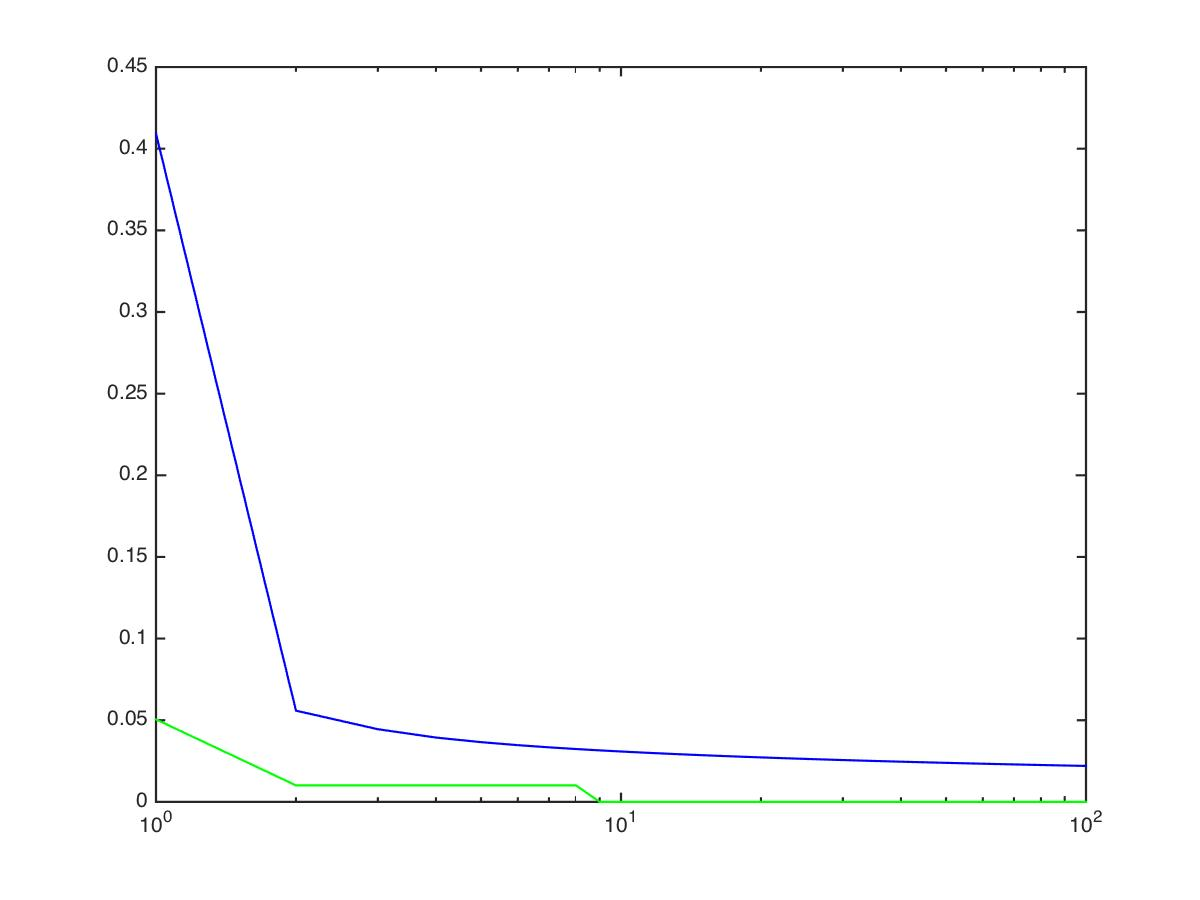
\includegraphics[scale=0.25]{logistic1.jpg}
}
\subfigure[Plot of the final converged classifier]{
    \label{fig:logisticxa2}
    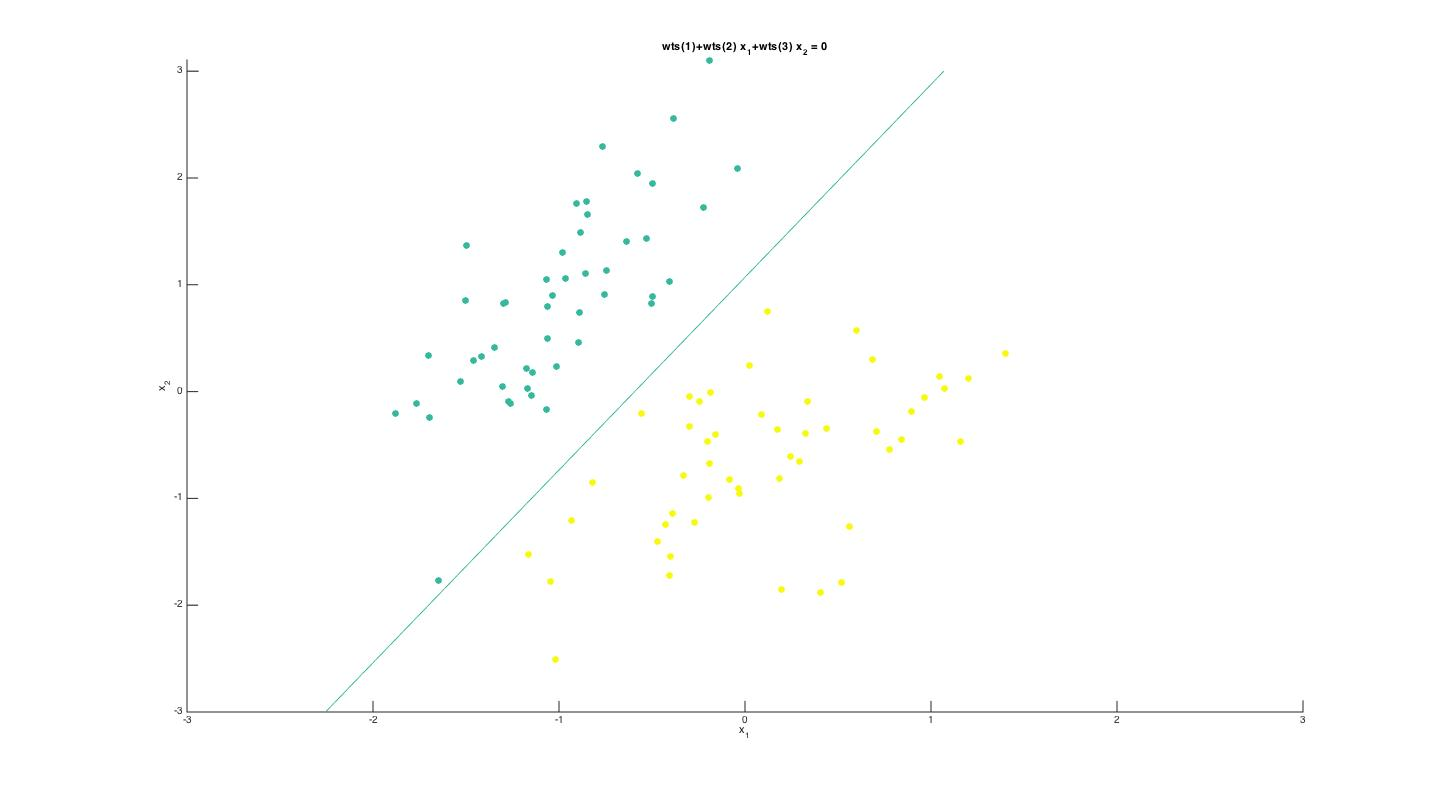
\includegraphics[scale=0.25]{logistic2.jpg}
}
\subfigure[final converged classifier decision boundaries]{
    \label{fig:logisticxa2}
    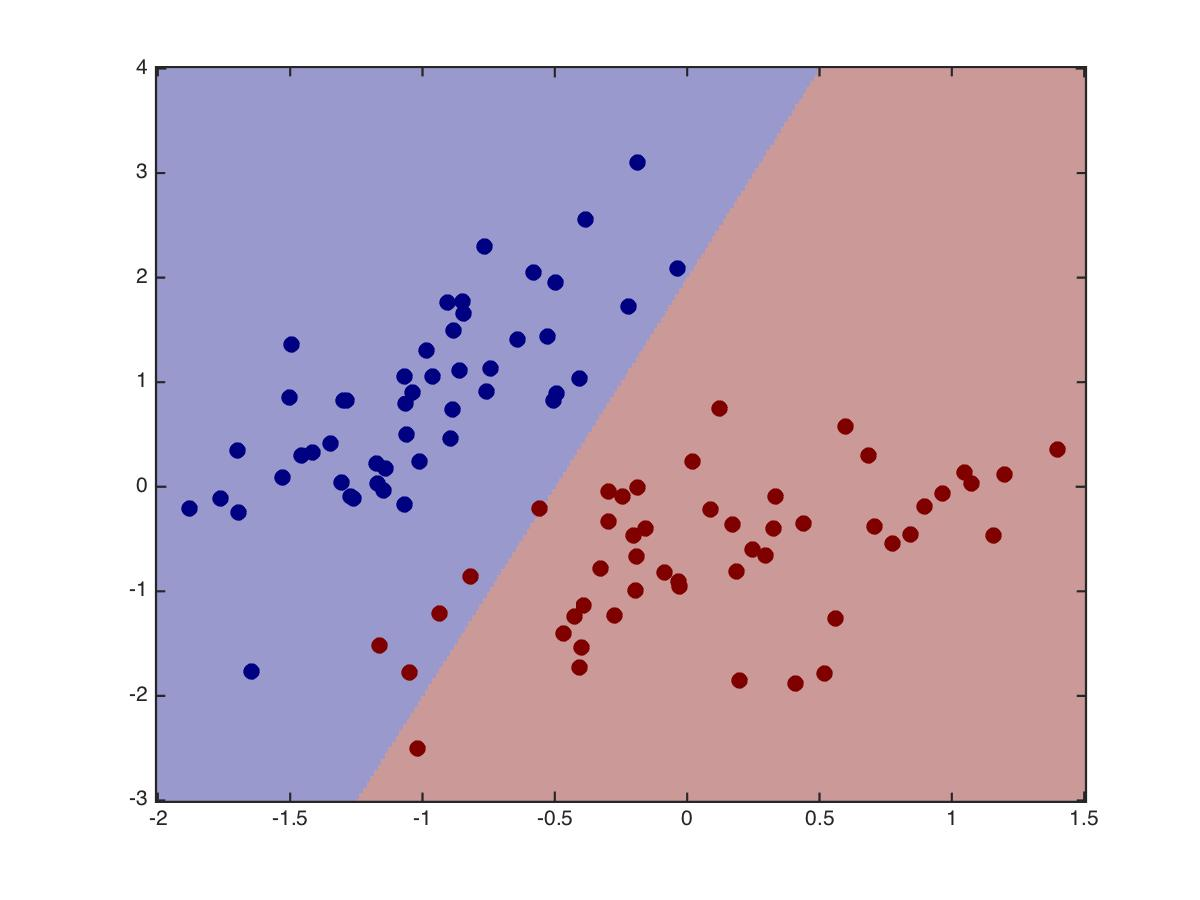
\includegraphics[scale=0.25]{logisticclassifyxa.jpg}
}
\caption[Scatter]{For data \mcode{XA}, the error, surrogate loss plots and the classes.}
\label{fig:logisticxa}
\end{figure}

\begin{figure}
\centering
\subfigure[Plot of convergence of the surrogate loss and the error rate]{
    \label{fig:logisticxb1}
    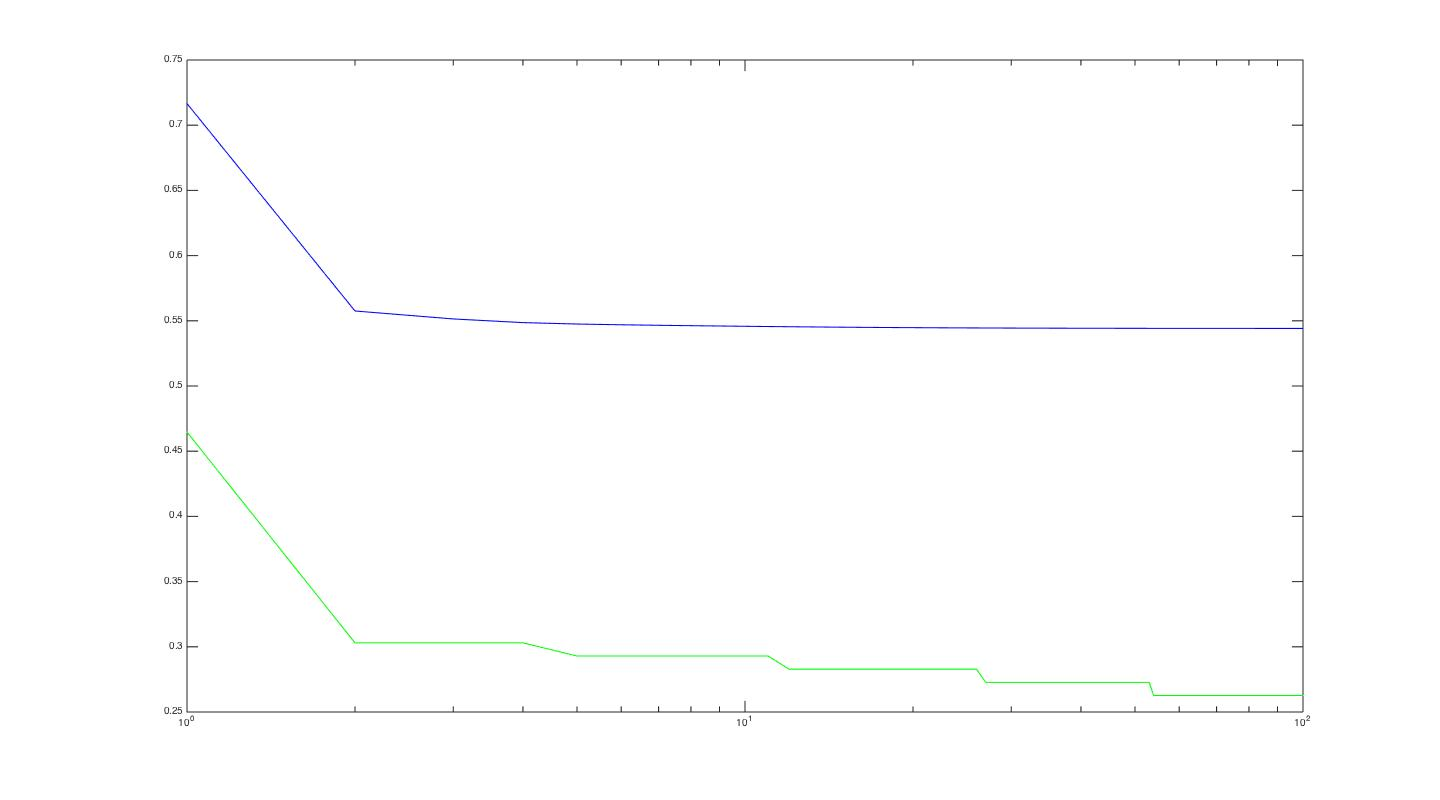
\includegraphics[scale=0.25]{logistic4.jpg}
}
\subfigure[Plot of the final converged classifier]{
    \label{fig:logisticxb2}
    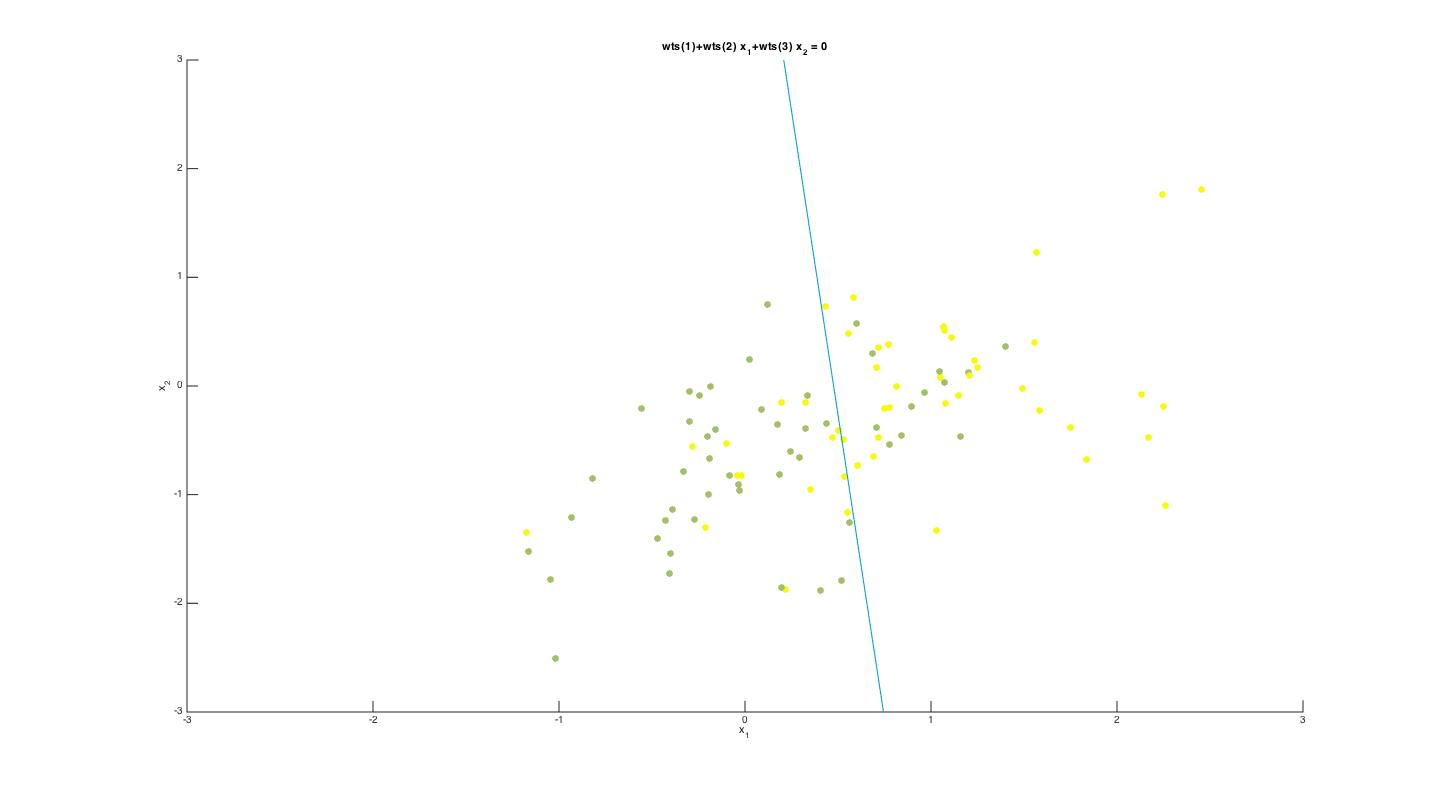
\includegraphics[scale=0.25]{logistic3.jpg}
}
\subfigure[final converged classifier decision boundaries]{
    \label{fig:logisticxa2}
    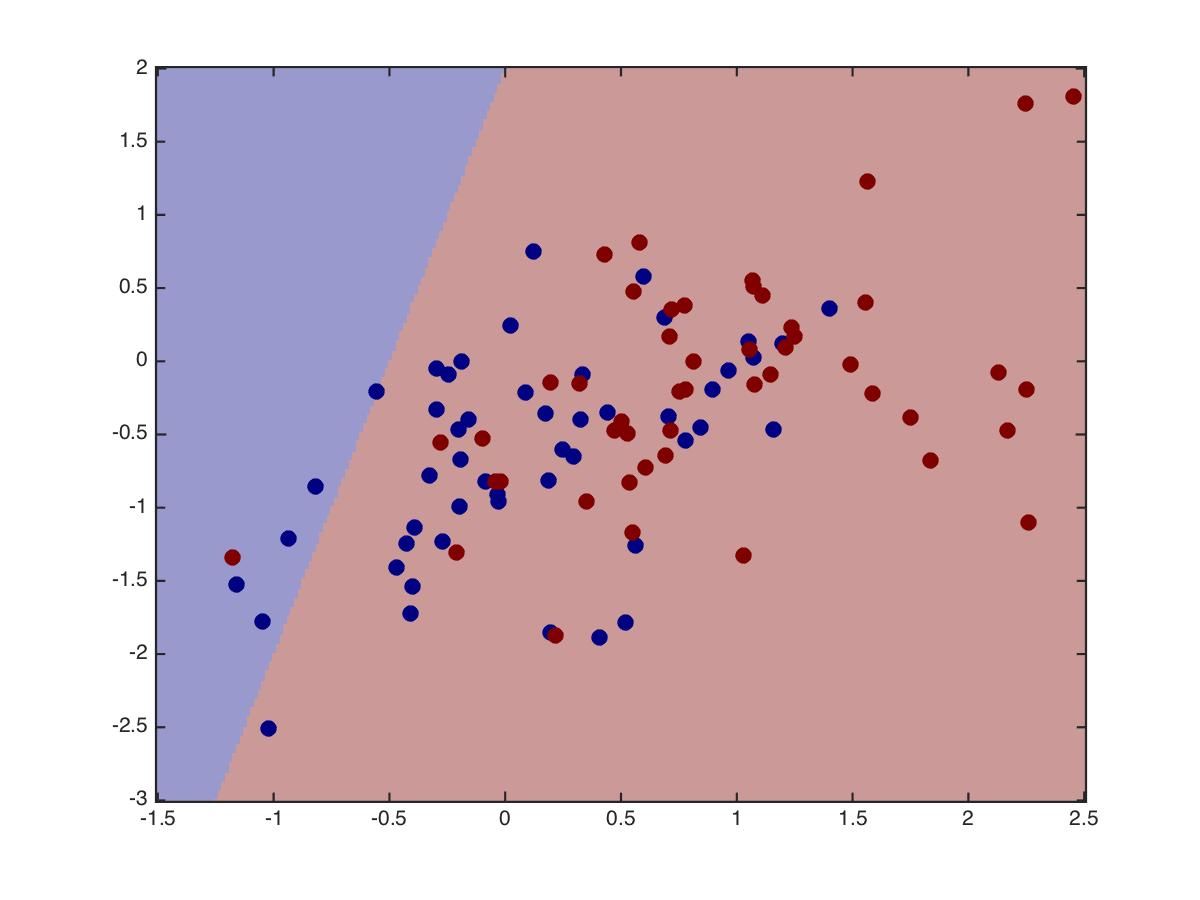
\includegraphics[scale=0.25]{logisticclassifyxb.jpg}
}
\caption[Scatter]{For data \mcode{XB}, the error, surrogate loss plots and the classes.}
\label{fig:logisticxb}
\end{figure}
\end{enumerate}

%%%%%%%%%%%%%%%%%%%%%%%%%%%%%%%%%%%%%%%%%%%%%%%%%%%%%%%%%
%%%%%%%%%%%%%%%%%%%%%%%%%%%%%%%%%%%%%%%%%%%%%%%%%%%%%%%%%
\pagebreak
\section*{Problem 2: Shattering and VC Dimensions}
\vspace{-10pt}

\begin{enumerate}[(a)]
\item \(T(a+bx_1)\) : This function presents a line with the slope to be \(b\) and interception to be \(a\). It would be able to shatter the cases (a), (b),  and (c). 
\begin{itemize}
\item It would be able to shatter the case (a) as a line can be on either sides of the single point and classify it in distinct classes.
\item It would be able to shatter the case (b) as the line can be on either sides of the two points and in the middle to classify both the points as +1, or -1 or into two separate classes.
\item It would be able to shatter the case (c) as the line can be on either sides of the three points. The advantage of interceptions and slope is that the line representing the decision boundary could be placed anywhere.
\end{itemize}
The (d) case would not be shattered by the line as it would not be able to divide the points where the classes of the diagonal points are same. It can be seen in \autoref{fig:shatter1d}.

\begin{figure}
\centering
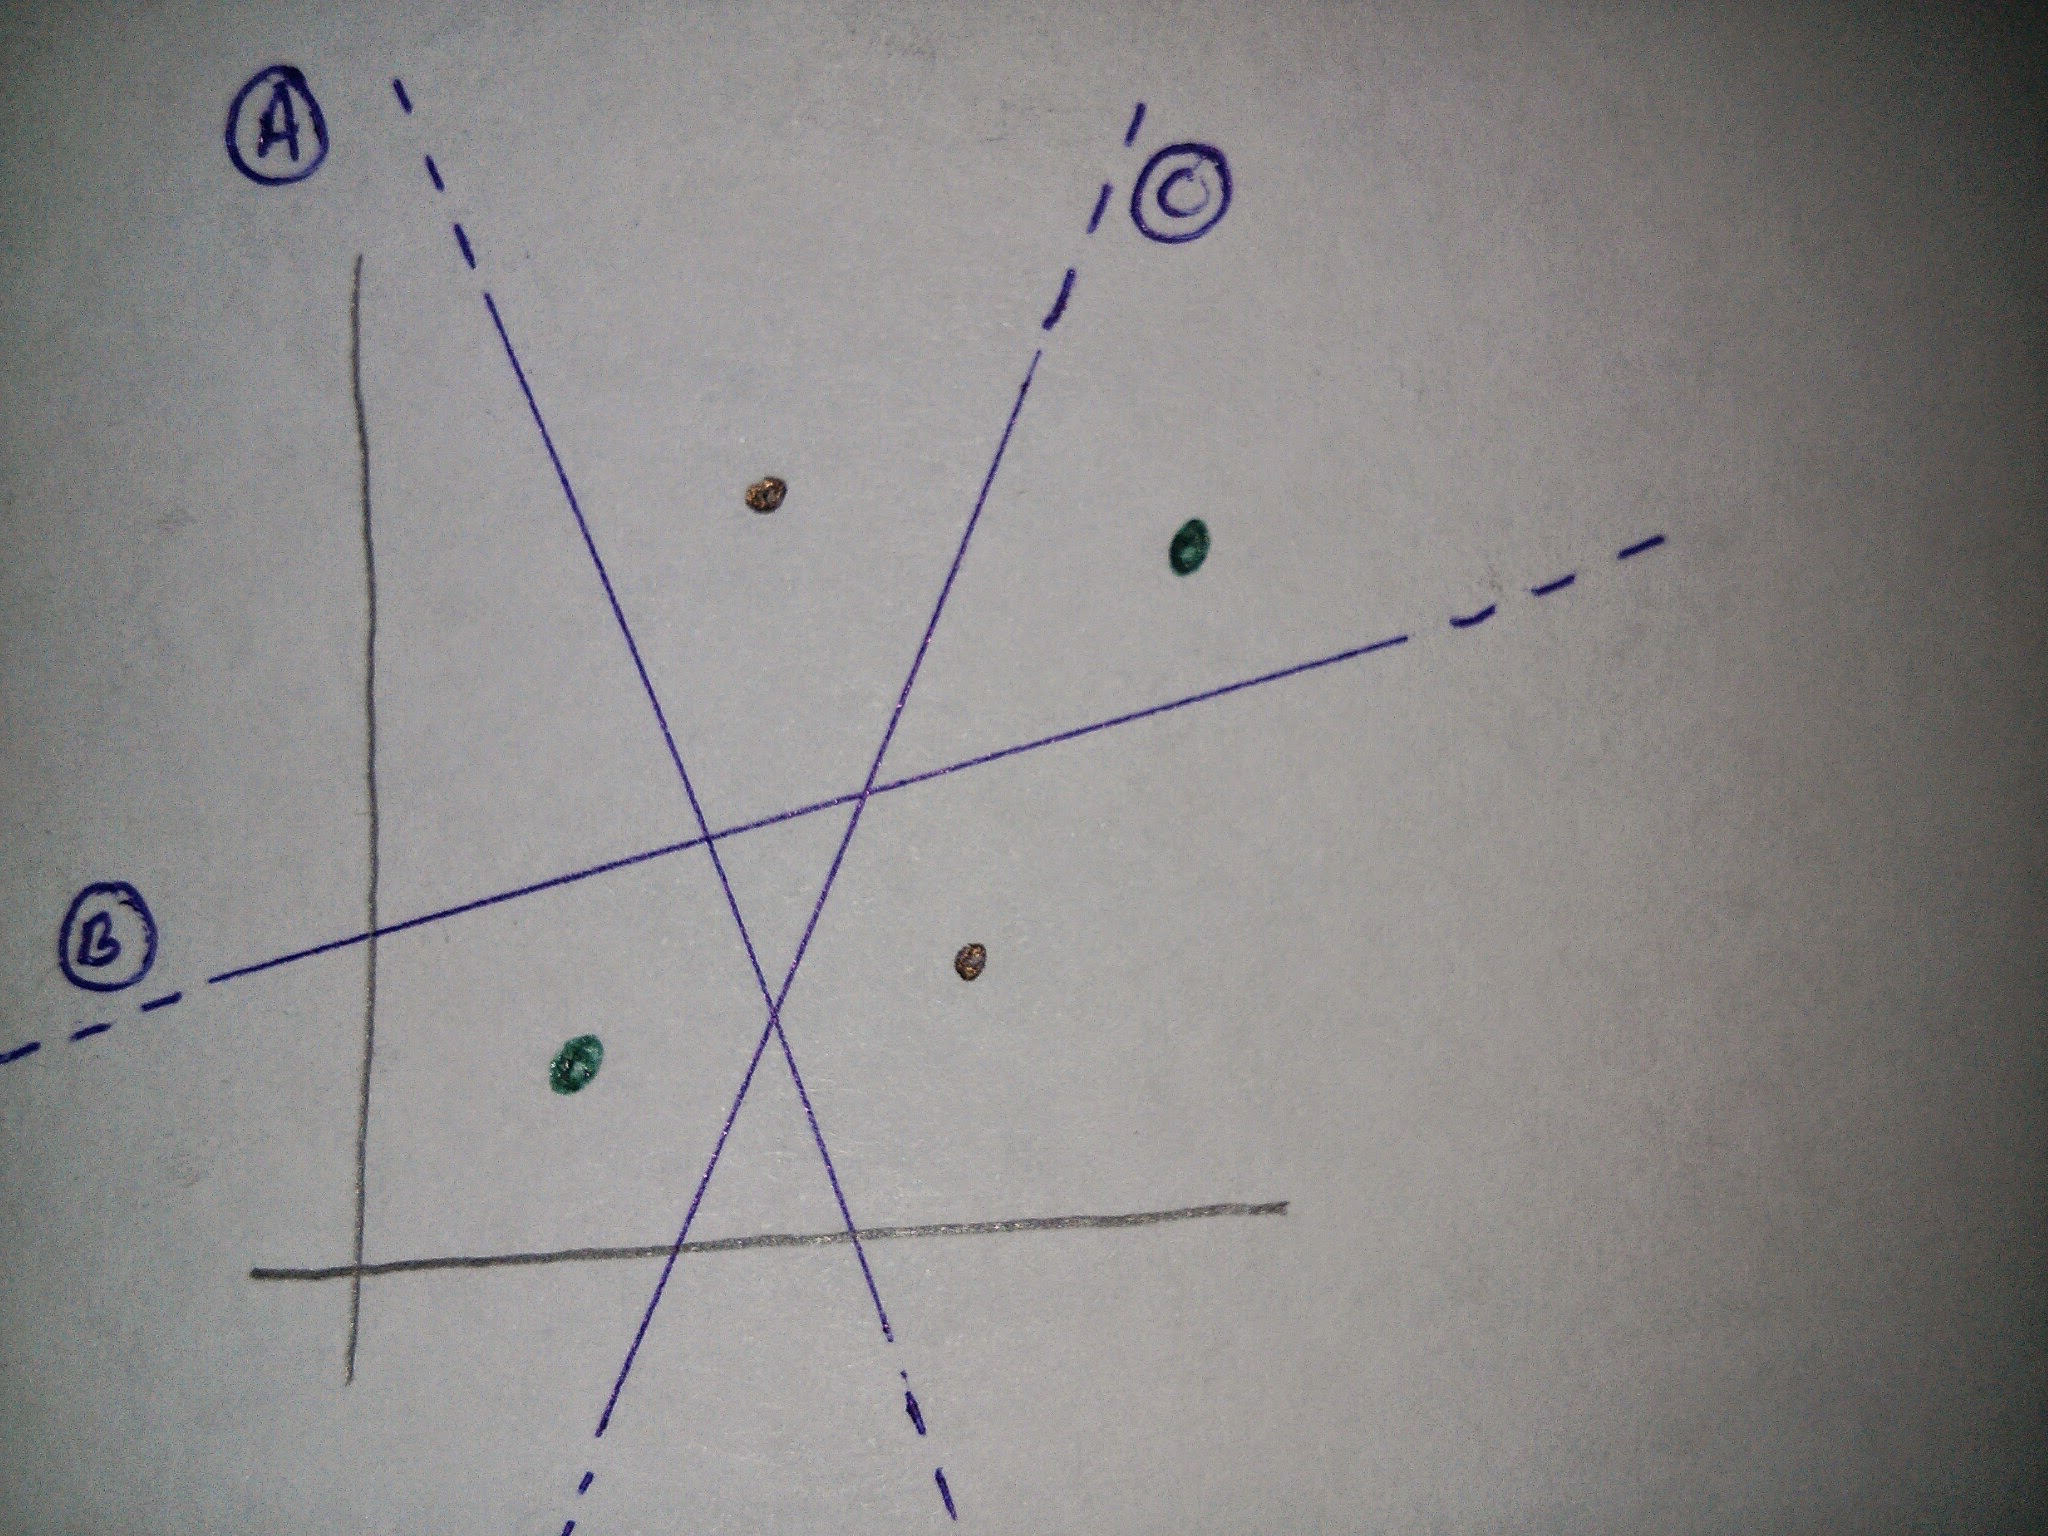
\includegraphics[scale=0.15]{shatter1.jpg}
\caption[Example Problem and Solution]{A, B, and C lines (representing the decision boundaries) trying to shatter 4 points with diagonal points with the same classes.}
\label{fig:shatter1d}
\end{figure}

\item \(T((x_1 - a)^2 + (x_2 - b)^2 + c)\) : This function presents a circle with coordinates of the center \((a,b)\). It would be able to shatter the cases (a), (b). 
\begin{itemize}
\item It would be able to shatter the case (a) as either the lone point can be inside the circle or outside it, representing two different classes.
\item It would be able to shatter the case (b) as the line as either the two points could be inside the circle, or outside the circle. Small circle can also be drawn to only contain individual points.
\end{itemize}
The (c) case would not be shattered by the circle as the placement of the three points would not allow a circle to be formed in a way that only two points come A and B come inside the circle and not C as can be seen in \autoref{fig:shatter2c2}. The (d) case have similar problem, with two points.
\begin{figure}
\centering
\subfigure[Calculations of the distances computed amongst the points]{
\label{fig:shatter2c1}
    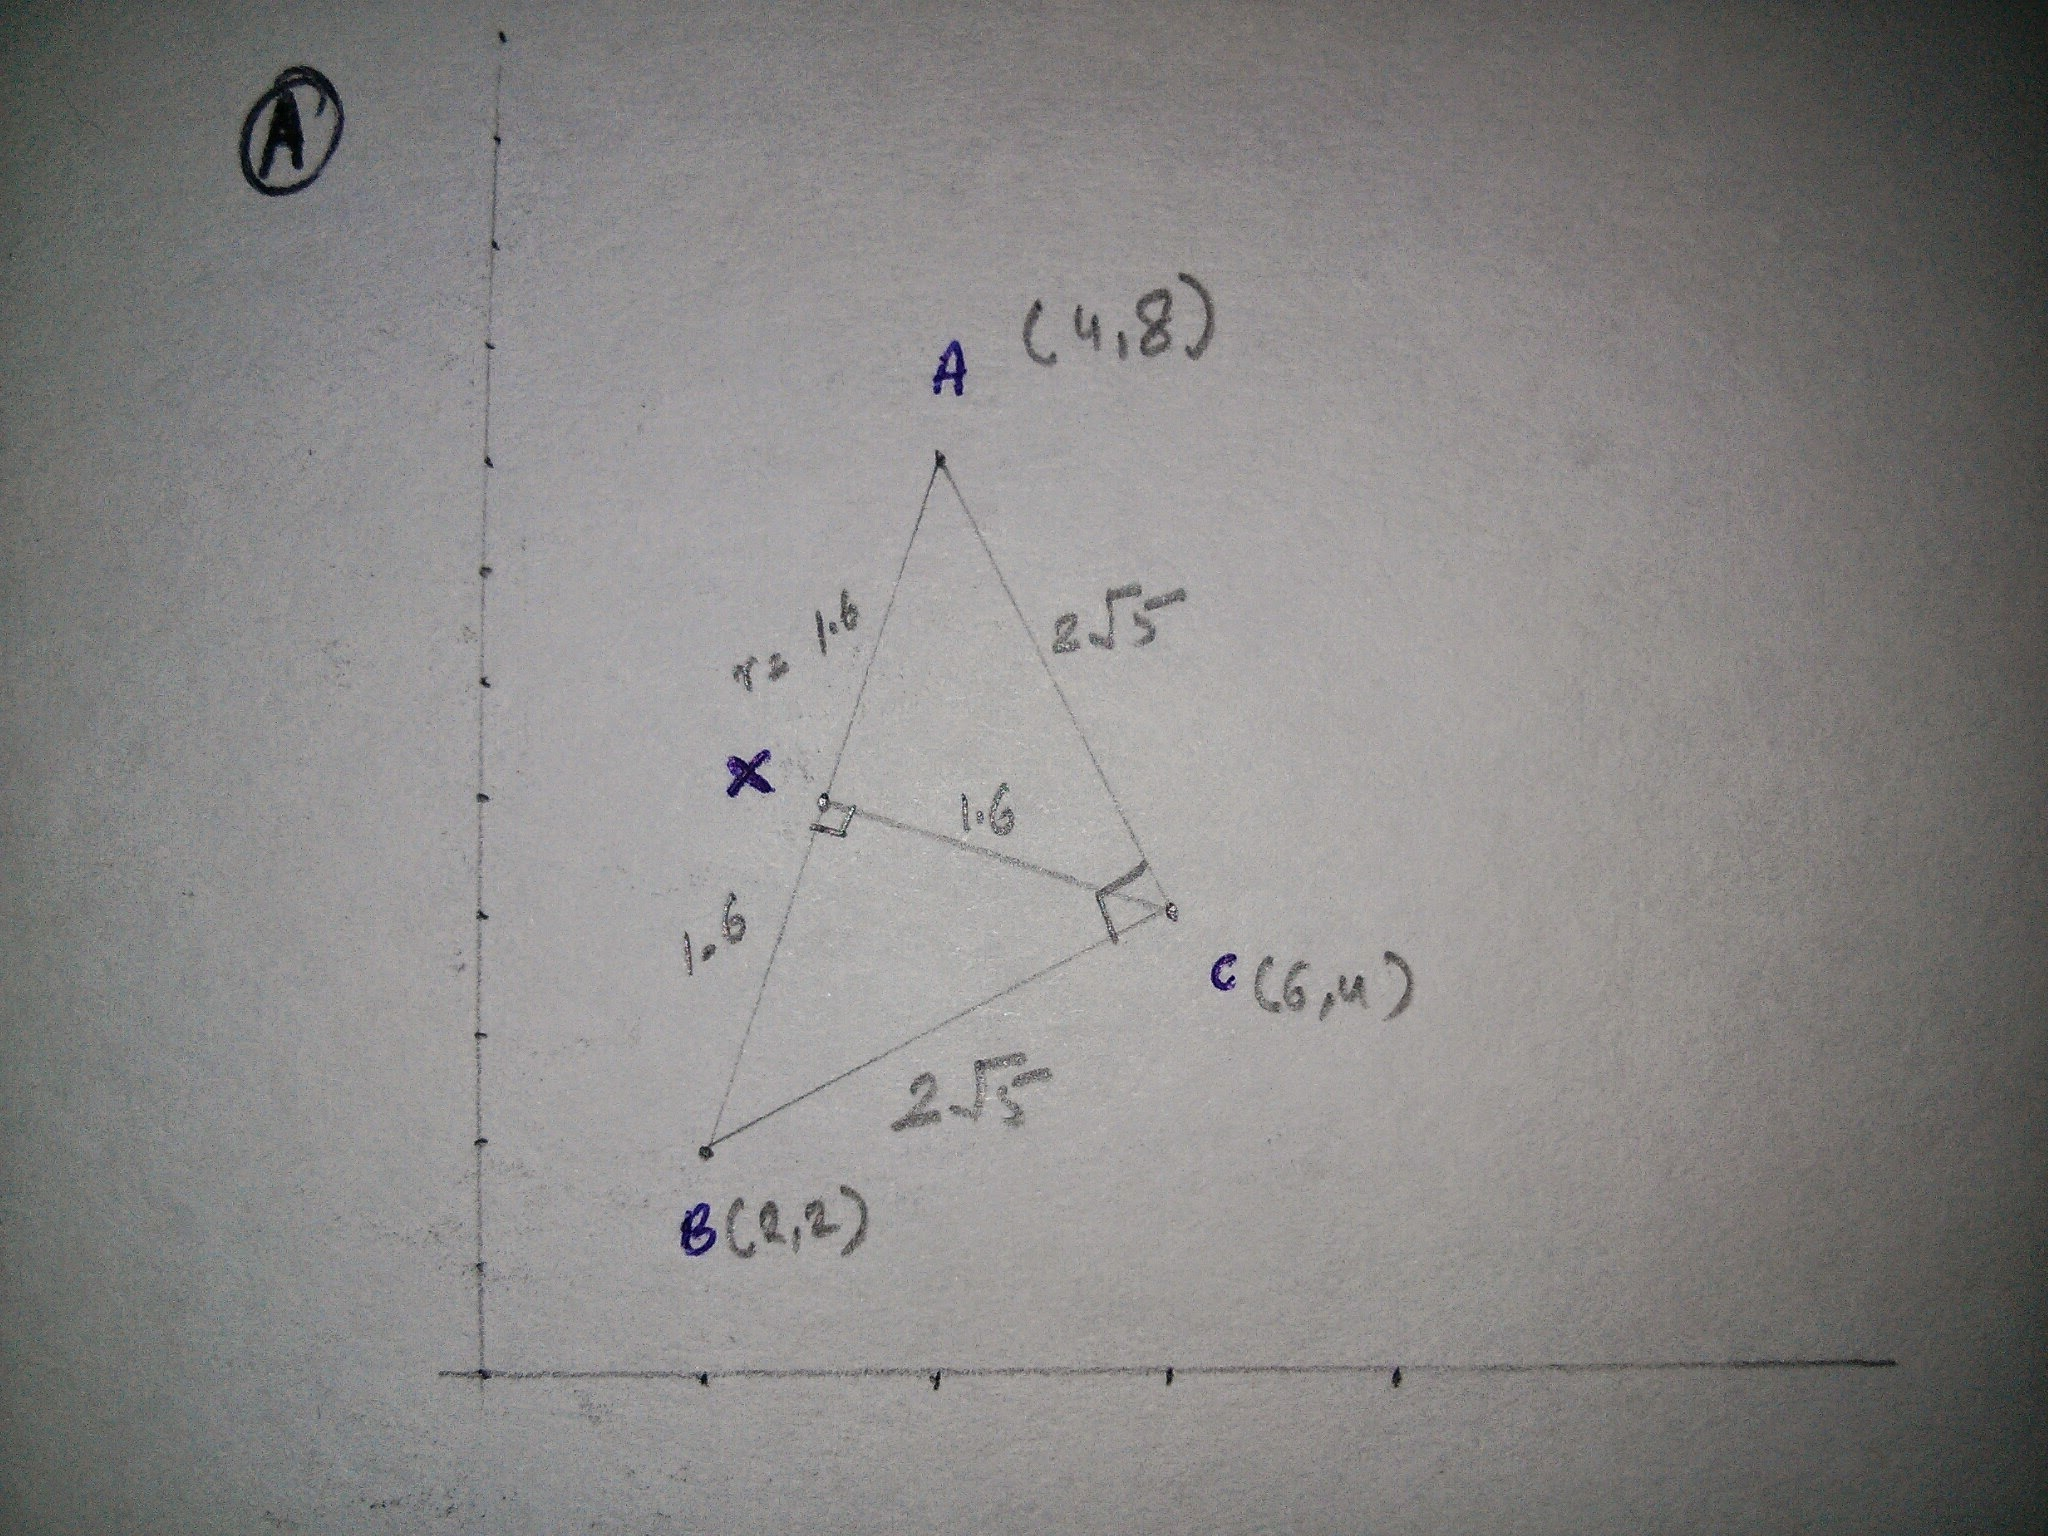
\includegraphics[scale=0.20]{shatter2.jpg}
}
\subfigure[Trying to shatter placing a circle with A and B being two-ends of the diameter]{
\label{fig:shatter2c2}
    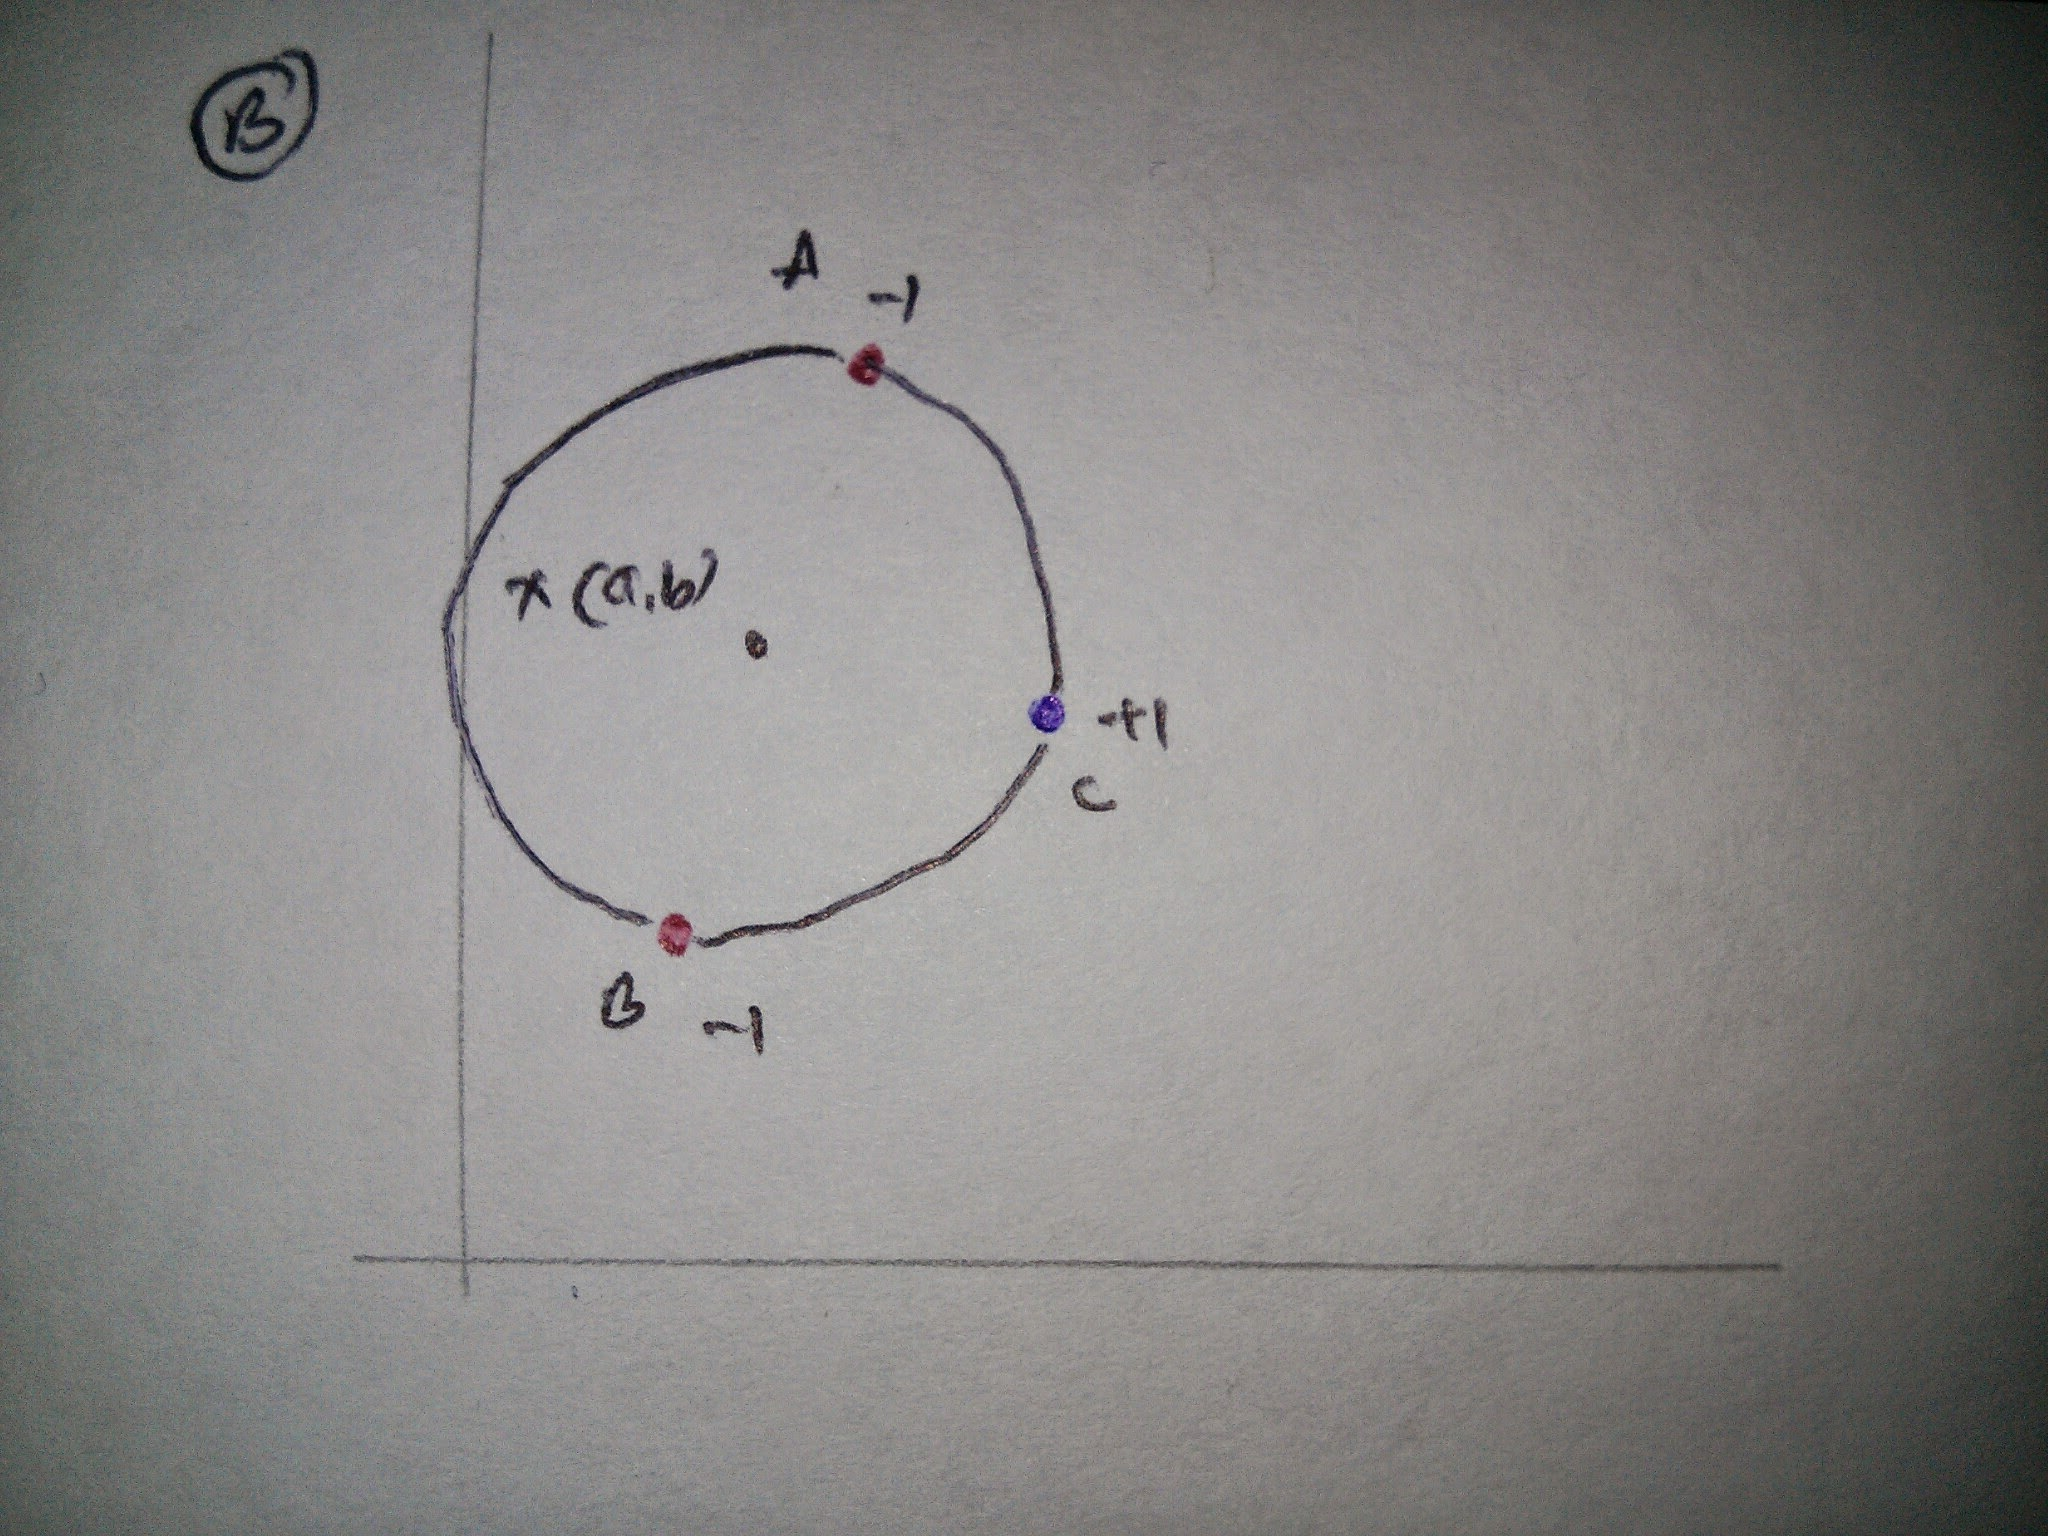
\includegraphics[scale=0.20]{shatter3.jpg}
}
\caption[Scatter]{Trying to shatter with circle. The calculations for the distances are shown in \autoref{fig:shatter2c1}.}
\label{fig:shatter2c}
\end{figure}

\item \(T((a * b)x_1 + (c/a)x_2)\) : This function shows lines passing through the origin. It would be able to shatter the cases (a), (b). 
\begin{itemize}
\item It would be able to shatter the case (a) as a line can be on either sides of the single point and classify it in distinct classes.
\item It would be able to shatter the case (b) as the line can be on either sides of the two points and in the middle to classify both the points as +1, or -1 or into two separate classes.
\end{itemize}
The (c) case would not be shattered by the line passing through the origin as the lines would not be able to separate points with same classes on one side, such as X, and Z in the \autoref{fig:shatter3c}. The configurations A, B, C and D show the various situations where the function fails to shatter the points. The same is true for the case (d) where the fourth point would not be shattered.
\begin{figure}
\centering
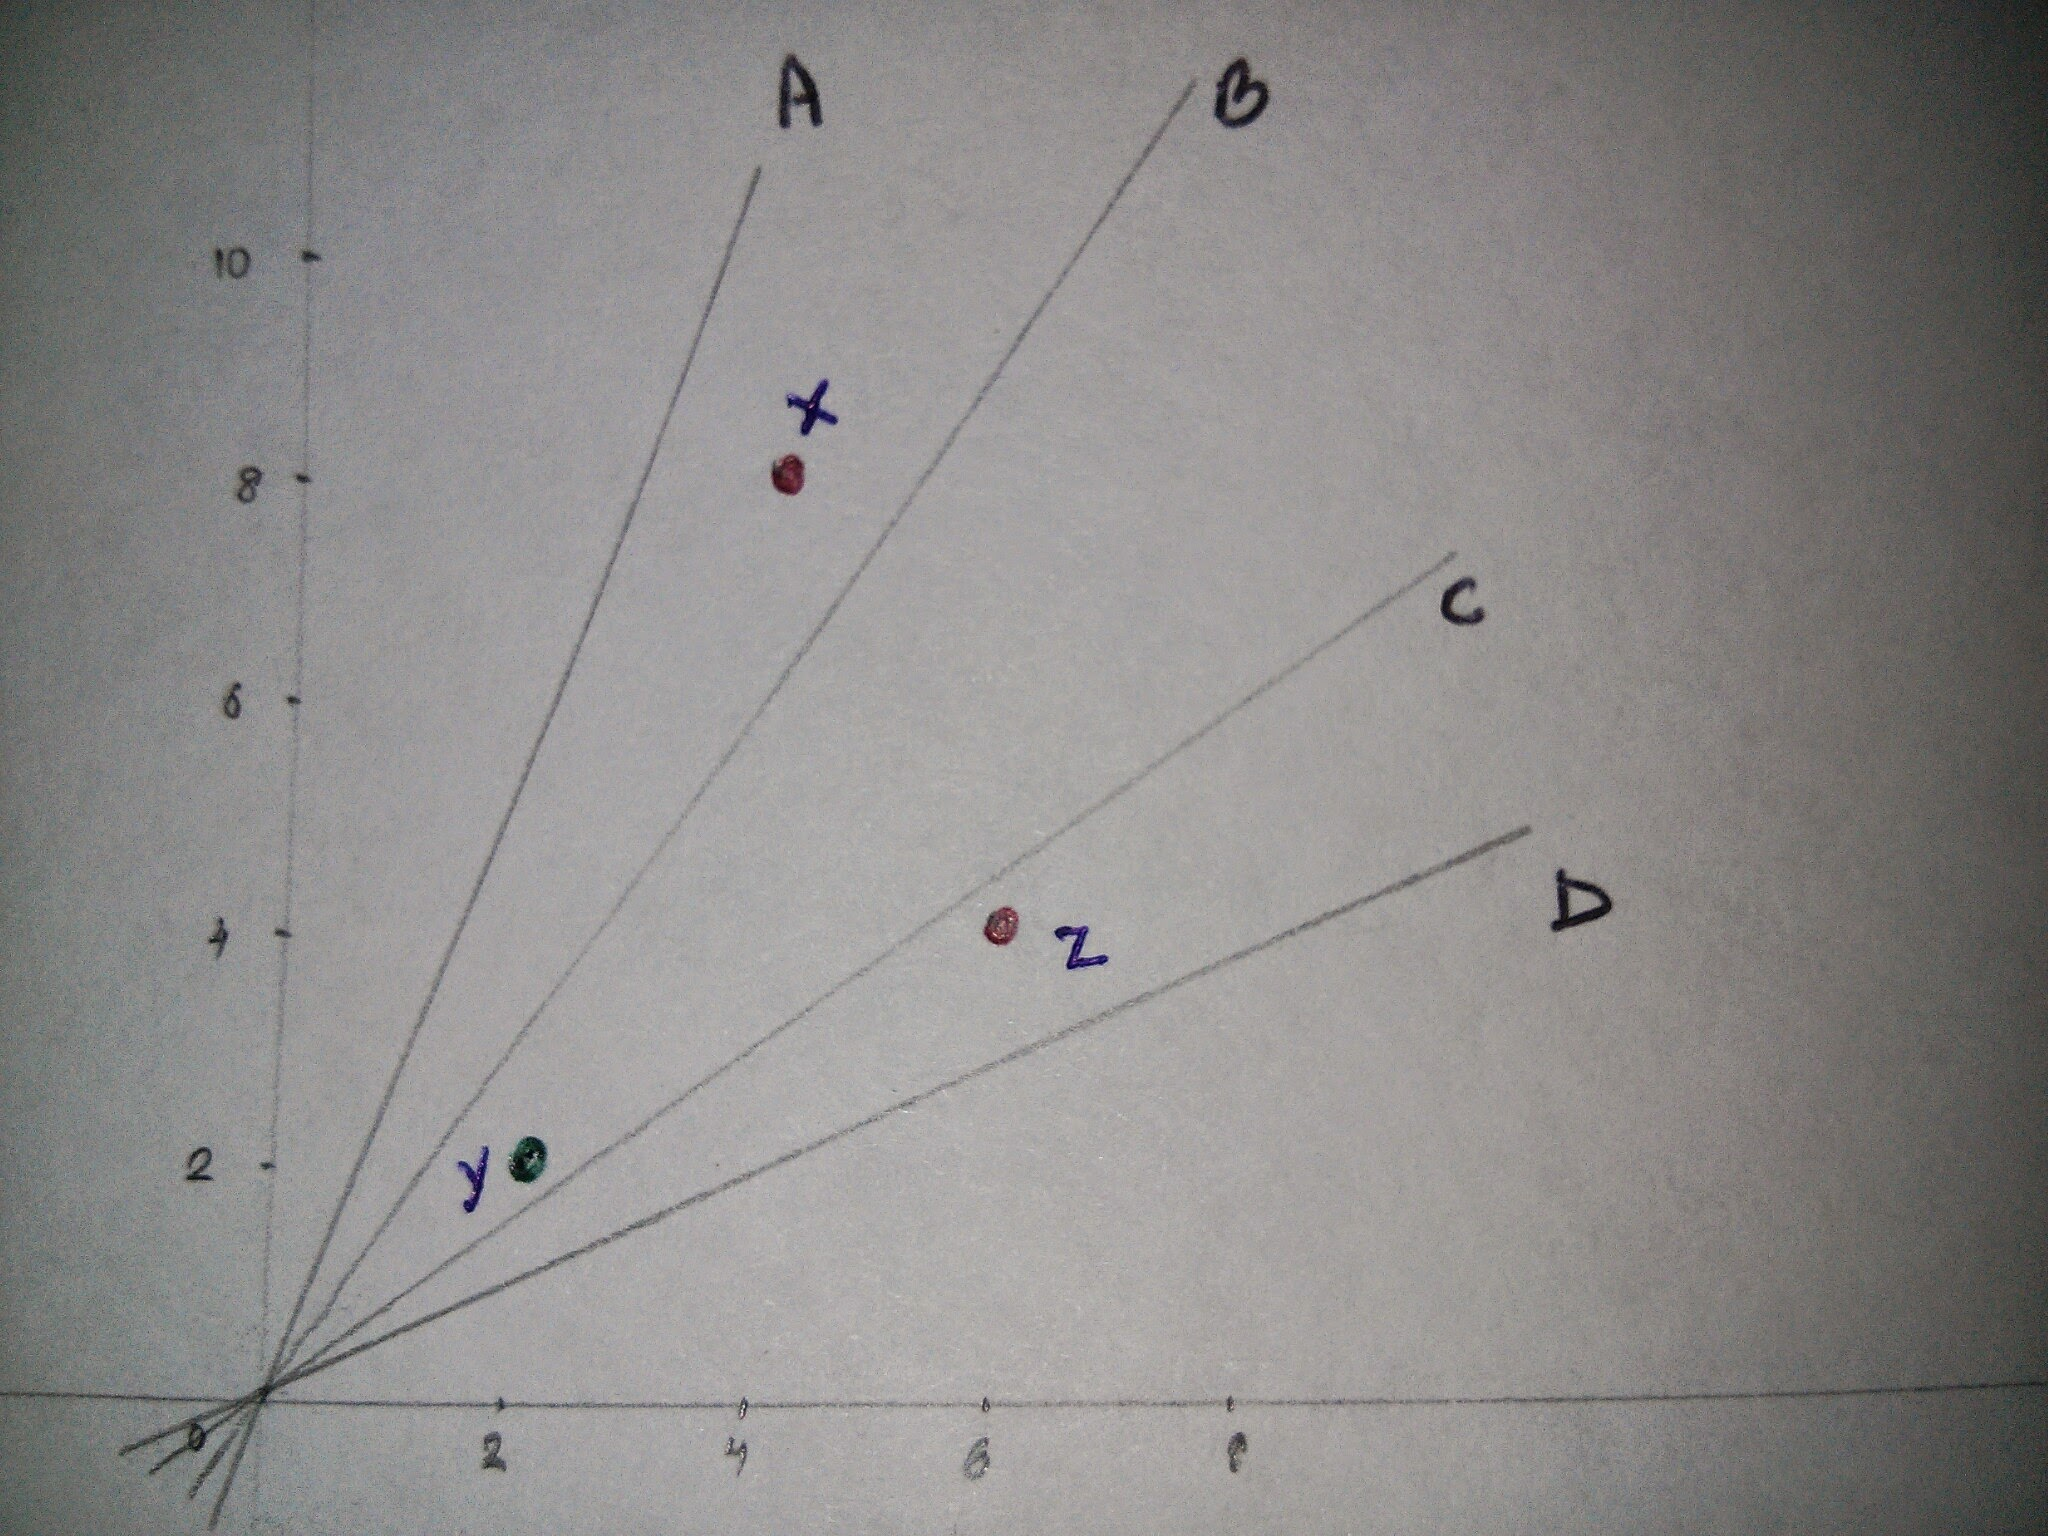
\includegraphics[scale=0.20]{shatter4.jpg}
\caption[]{The lines A, B, C and D represent various function values.}
\label{fig:shatter3c}
\end{figure}
\end{enumerate}
\end{document}

%%%%%%%%%%%%%%%%%%%%%%%%%%%%%%%%%%%%%%%%%%%%%%%%%%%%%%%%%
%%%%%%%%%%%%%%%%%%%%%%%That's all folks%%%%%%%%%%%%%%%%%%%%%%%%%%%
%%%%%%%%%%%%%%%%%%%%%%%%%%%%%%%%%%%%%%%%%%%%%%%%%%%%%%%%%
\iffalse
\begin{figure}
\centering
\subfigure[Puzzle 1]{
    \label{fig:subfig1}
    \includegraphics[scale=0.30]{g1.png}
}
\subfigure[Puzzle 2]{
    \label{fig:subfig2}
    \includegraphics[scale=0.30]{g2.png}
}
\subfigure[Puzzle 3]{
    \label{fig:subfig3}
    \includegraphics[scale=0.30]{g3.png}
}
\subfigure[Puzzle 4]{
    \label{fig:subfig4}
    \includegraphics[scale=0.30]{g4.png}
}
\subfigure[Puzzle 5]{
    \label{fig:subfig5}
    \includegraphics[scale=0.30]{g5.png}
}
\subfigure[Puzzle 6]{
    \label{fig:subfig6}
    \includegraphics[scale=0.30]{g6.png}
}
\caption[Running Various Experiments]{Running Various Experiments. The three bars are for Brute Force, I-Consistency and I-Consistency with MRV search. All the times given are in Seconds}
\label{fig:rungraphs}
\end{figure}

\begin{figure}
\centering
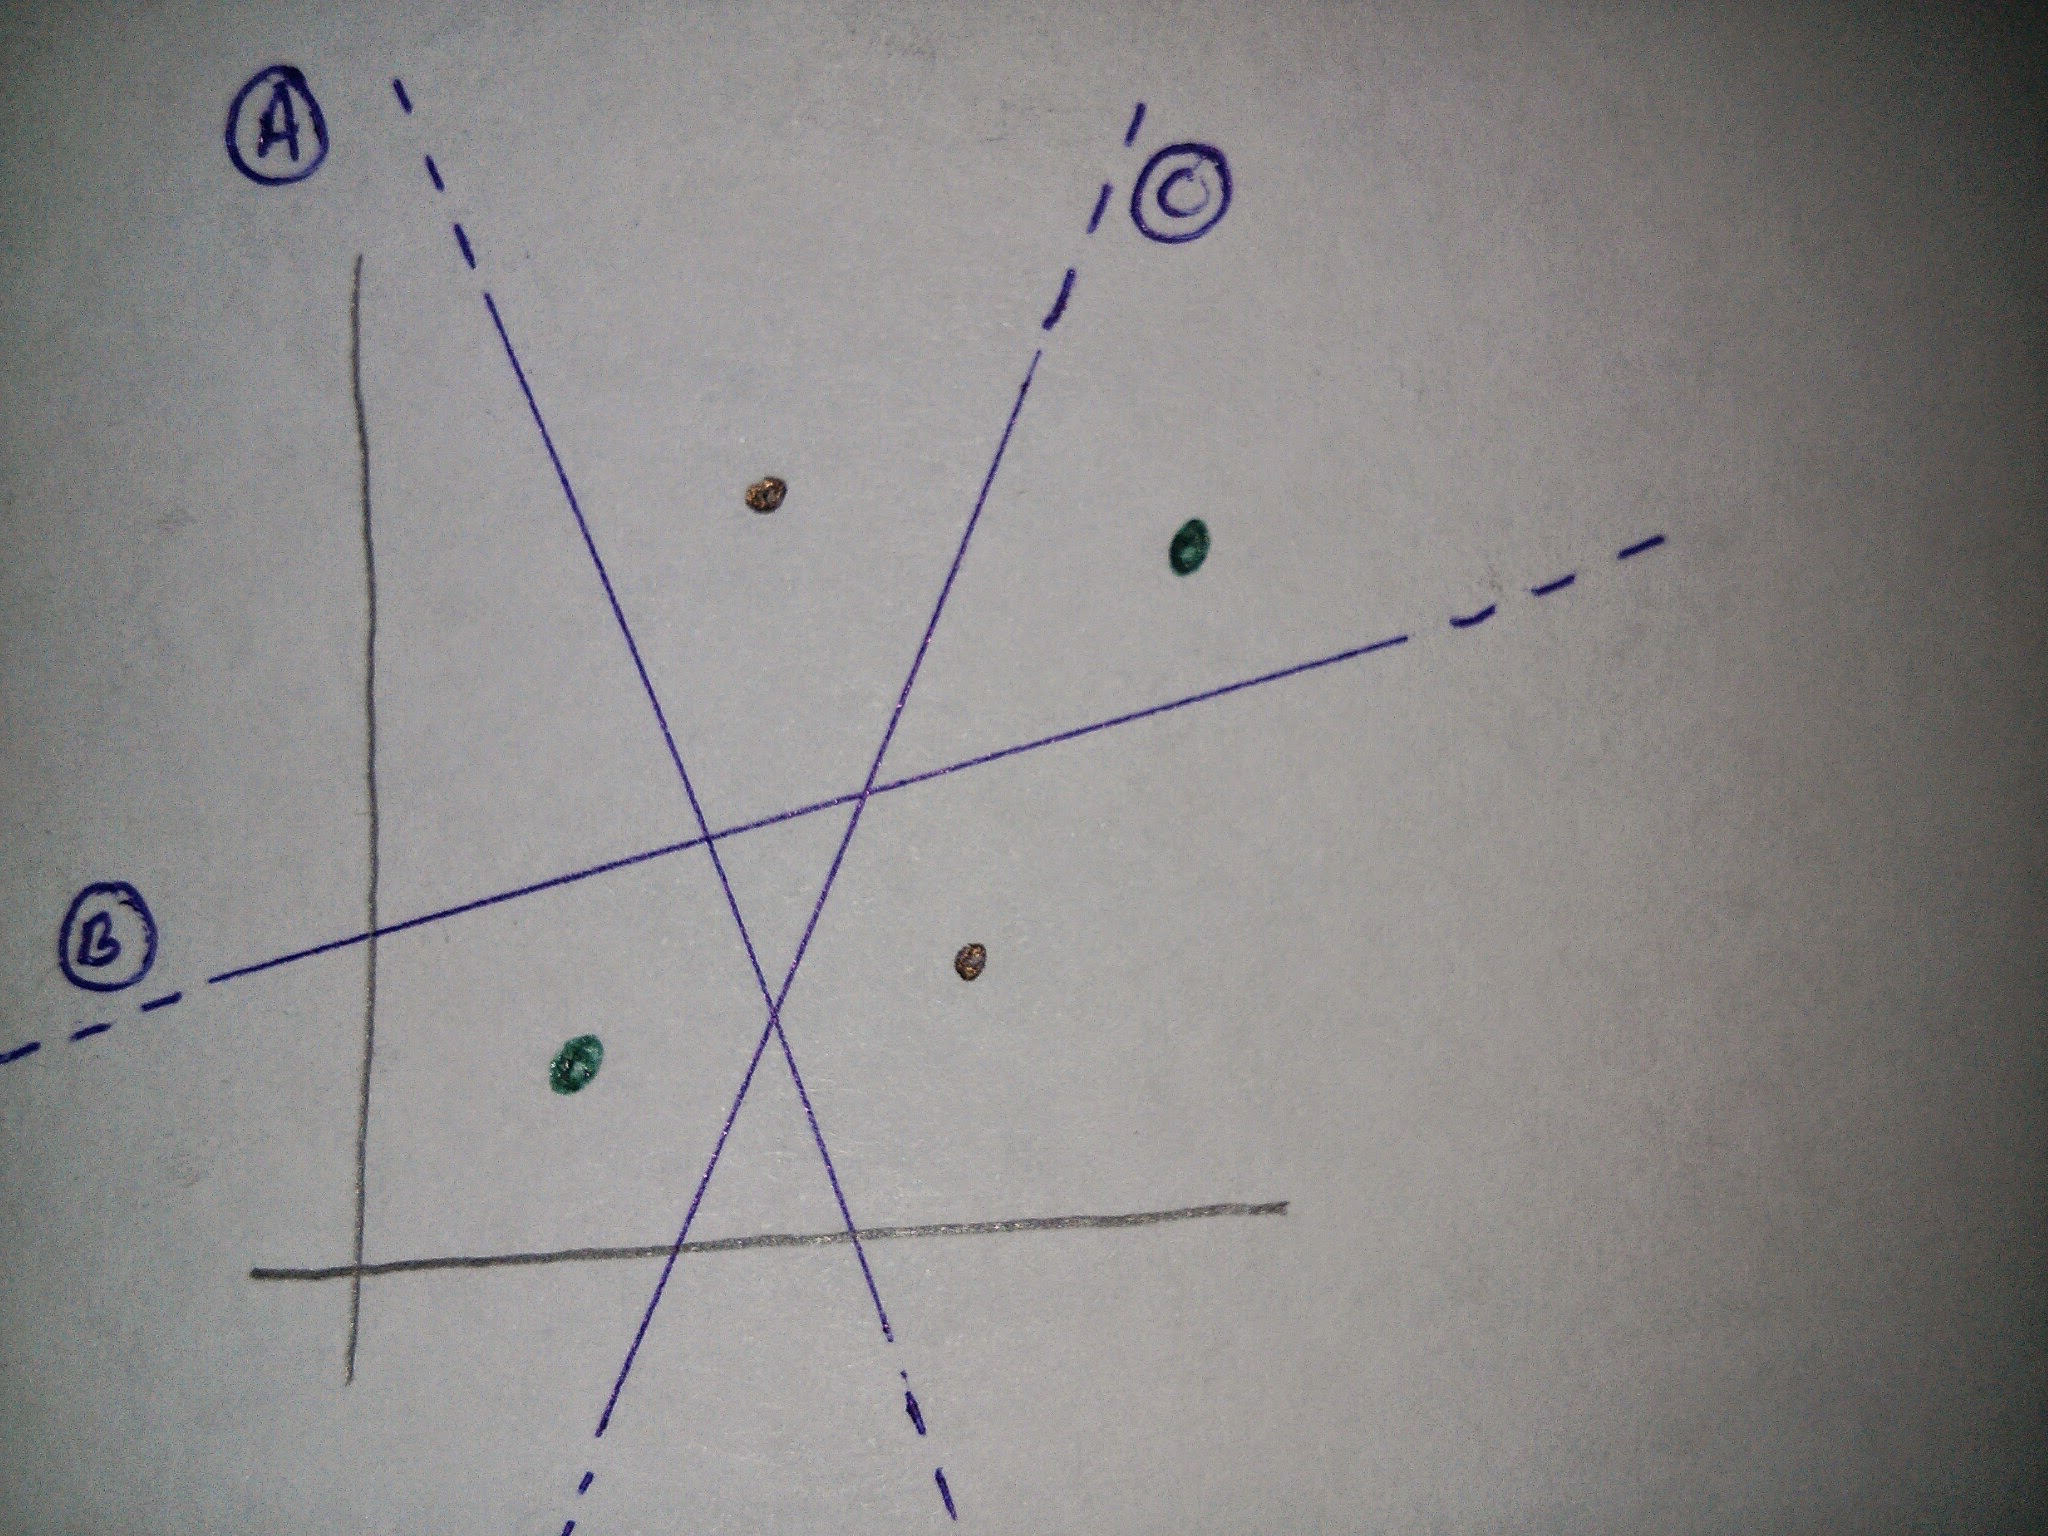
\includegraphics[scale=0.15]{shatter1.jpg}
\caption[Example Problem and Solution]{Example Problem and Solution}
\label{fig:kakuroExample}
\end{figure}

\begin{lstlisting}[caption={Training linear regression with cross-validation.},label={lst:cv1},numbers=left,escapeinside={@}{@}]
%%% MATLAB Code.
i = 1;
nFolds = 5;
d=[1,3,5,7,10,18];
\end{lstlisting}

\fi